\documentclass[11pt]{article}
\usepackage[utf8]{inputenc}
\usepackage{color, hyperref, amsmath, graphicx, Rd}
\usepackage{framed}
\usepackage{alltt}

\setlength{\oddsidemargin}{0in} \setlength{\textwidth}{6.5in}
\setlength{\topmargin}{0in} \setlength{\textheight}{8.5in}
\setlength{\textwidth}{6.5in} \setlength{\textheight}{8.5in}

\makeatletter
\def\maxwidth{ %
  \ifdim\Gin@nat@width>\linewidth
    \linewidth
  \else
    \Gin@nat@width
  \fi
}
\makeatother

\definecolor{fgcolor}{rgb}{0.345, 0.345, 0.345}
\newcommand{\hlnum}[1]{\textcolor[rgb]{0.686,0.059,0.569}{#1}}%
\newcommand{\hlstr}[1]{\textcolor[rgb]{0.192,0.494,0.8}{#1}}%
\newcommand{\hlcom}[1]{\textcolor[rgb]{0.678,0.584,0.686}{\textit{#1}}}%
\newcommand{\hlopt}[1]{\textcolor[rgb]{0,0,0}{#1}}%
\newcommand{\hlstd}[1]{\textcolor[rgb]{0.345,0.345,0.345}{#1}}%
\newcommand{\hlkwa}[1]{\textcolor[rgb]{0.161,0.373,0.58}{\textbf{#1}}}%
\newcommand{\hlkwb}[1]{\textcolor[rgb]{0.69,0.353,0.396}{#1}}%
\newcommand{\hlkwc}[1]{\textcolor[rgb]{0.333,0.667,0.333}{#1}}%
\newcommand{\hlkwd}[1]{\textcolor[rgb]{0.737,0.353,0.396}{\textbf{#1}}}%

\makeatletter
\newenvironment{kframe}{%
 \def\at@end@of@kframe{}%
 \ifinner\ifhmode%
  \def\at@end@of@kframe{\end{minipage}}%
  \begin{minipage}{\columnwidth}%
 \fi\fi%
 \def\FrameCommand##1{\hskip\@totalleftmargin \hskip-\fboxsep
 \colorbox{shadecolor}{##1}\hskip-\fboxsep
     % There is no \\@totalrightmargin, so:
     \hskip-\linewidth \hskip-\@totalleftmargin \hskip\columnwidth}%
 \MakeFramed {\advance\hsize-\width
   \@totalleftmargin\z@ \linewidth\hsize
   \@setminipage}}%
 {\par\unskip\endMakeFramed%
 \at@end@of@kframe}
\makeatother

\definecolor{shadecolor}{rgb}{.97, .97, .97}
\definecolor{messagecolor}{rgb}{0, 0, 0}
\definecolor{warningcolor}{rgb}{1, 0, 1}
\definecolor{errorcolor}{rgb}{1, 0, 0}
\newenvironment{knitrout}{}{} % an empty environment to be redefined in TeX

%% for inline R code: if the inline code is not correctly parsed, you will see a message
\newcommand{\rinline}[1]{SOMETHING WRONG WITH knitr}

\title{STAT 243: \\
	Model Selection with\\ 
	Genetic Algorithms using \texttt{GA}}
\author{Eddie Buehler, Yang Hu \& Jin Rou New\\
	University of California, Berkeley}

\date{Version 1.0, \today}

\setlength\parindent{0pt}
\setlength{\parskip}{\baselineskip}% to get space between paragraphs


\begin{document}
\maketitle

\section{Introduction}
\label{sec:introduction}
A genetic algorithm is an optimization technique that mimics the
biological process of natural selection. The basic strategy is to take
a population of candidate solutions and ``evolve" them over many generations towards an
optimal solution. Continuing the biology analogy, the
population is typically represented as a collection of a series of bits called chromosomes. A fitness function is evaluated at each iteration to
determine how well the current population of chromosomes solves the objective
function. A genetic algorithm has the following steps: 
\begin{enumerate}
	\item Calculate fitness of chromosomes. Often, the
          fitness is the value of the objective function solving the
          optimization. The better the fitness, the better solution
          the chromosomes will provide.
	\item Select chromosomes to form a mating pool based on their
          fitness. This process is performed stochastically, with more
          fit chromosomes having a higher probability of being
          selected. 
	\item Recombine parent chromosomes from the mating pool. This
          is the first step in producing the next generation of
          chromosomes in which the parents' genes are combined.
	\item Apply mutation to produce the resulting generation of
          chromosomes. After crossover, each gene in the resulting
          population has a finite probability to flip its value.
    \item Repeat until either a set number of generations is reached.
\end{enumerate}

\section{Code}
\label{sec:code}
We took the S3 approach to object-oriented programming for our package and created functions that were as modular as possible to facilitate code creation, maintenance and testing.

For a given data set, e.g. the built-in \texttt{airquality} data set in \texttt{R}, the user can carry out model selection for an ordinary linear regression of the variable \texttt{Ozone} on other variables in the data set with the main function in the package as follows:
\begin{verbatim}
ga <- select(data = airquality, yvar = "Ozone")
\end{verbatim}

Finer control of other parameters in the genetic algorithm for model selection is possible by changing the other function arguments. More details can be found in the \texttt{GA} manual in the ~\nameref{sec:appendix}.

The output of the results can be viewed using the following commands:
\begin{verbatim}
summary(ga)
model(ga)
\end{verbatim}

The result of this function is an object of \texttt{GA} class that contains the settings, model data, final population of chromosomes/models, model evaluation values of this population and all results of model selection using the genetic algorithm.

In the genetic algorithmic approach to model selection, a population of models, i.e. chromosomes with number of genes equal to the number of model variables under consideration, and with each gene taking a value of 1 if the model variable is included and 0 otherwise, is first initialized. This population then undergoes many iterations of reproduction. In the reproduction stage, each model/chromosome is then evaluated based on the desired model selection criterion, e.g. Akaike's Information Criterion. Chromosomes are then selected into the mating pool based on how well they perform on the model selection criterion. 

Next, 2 parent chromosomes are randomly selected from the mating pool to form a child chromosome, with some probability of recombination/crossover occurring in the process. This is repeated until the desired number of child chromosomes for the next generation is reached. Finally, mutation is applied with a low probability to each gene in the population of child chromosomes. The resulting population of child chromosomes forms the next generation. The whole process is repeated for a desired number of iterations. The model/chromosome with the minimum value of the model evaluation criterion across all generations is then the best model.

The following subsections elaborate on the main subfunctions in the \texttt{GA} package; for more detailed documentation, please refer to the \texttt{GA} manual in the ~\nameref{sec:appendix}.

\subsection*{initialize function}
We sample uniformly from the set of \{0, 1\} with replacement as many genes as is required, i.e. the product of the number of variables under consideration and the population size desired, for the initial population of chromosomes.

\subsection*{evaluate function}
We compute the value of the model evaluation criterion for every model/chromosome in the population. The default model evaluation criterion is Akaike Information Criterion (AIC). The user can also choose to use Bayesian Information Criterion (BIC) or define his/her own function.

\subsection*{select\_for\_mating function}
The default selection method is ``rank'', which refers to Linear Rank Selection (LRS). In LRS, chromosomes are first given ranks $r_i$ for $i = 1, ..., n$, where $n$ is the number of chromosomes in the population. The chromosome with the best (minimum) model evaluation criterion is assigned a rank of $n$. Chromosomes are then selected into the mating pool randomly with probability proportional to their relative rank, until the desired size of the mating pool is reached. This is done with the following algorithm:
\begin{enumerate}
\item Calculate for each chromosome its probability to be selected, $p_i = \frac{r_i}{\sum\limits_{i=1}^n{r_i}}$. Since the best chromosome is given the largest rank, it also has a highest probability of being selected.
\item Calculate the cumulative probability for each chromosome to be selected, $pc_i = \sum\limits_{j=1}^i{p_j}$.
\item Generate a random number $u$ uniformly in the range [0, 1].
\item Select the chromosome with index $i$ if $pc_i < u < pc_{i+1}$
\item Repeat until the desired number of chromosomes in the mating pool is select.
\end{enumerate}

The alternative selection method is ``tournament'', which refers to Tournament Selection. The idea is simple; in Tournament Selection, we randomly select 2 chromosomes from the population. The chromosome with the better model evaluation criterion is selected into the mating pool. This process is repeated (with replacement of both chromosomes each time) until the desired number of chromosomes in the mating pool is reached.

\subsection*{recombine function}
Recombination occurs with probability \texttt{prob\_recombine} for every set of 2 parent chromosomes; the child chromosome is simply a copy of the first parent chromosome if no recombination occurs. We implemented three methods of recombination: crossover at one point (``onepoint''), crossover at two points (``twopoint'') and uniform crossover (``uniform'').

For one-point crossover, a break point index $b$ is uniformly sampled from the set of \{1, ..., g\}, where $g$ is the number of genes on each chromosome. The resulting child chromosome then takes genes 1 to $b$ from the first parent and genes $b+1$ to $g$ from the second parent.

For two-point crossover, two break point indices $b_1$ and $b_2$ are uniformly sampled without replacement from the set of \{1, ..., g\}. The resulting child chromosome then takes genes 1 to $b_1$ from the first parent, genes $b_1+1$ to $b_2$ from the second parent, and finally genes $b_2+1$ to $g$ from the first parent.

For uniform crossover, the child chromosome has equal probability of receiving each gene from either parent.

\subsection*{mutate function}
We generate as many Bernoulli variables as there are genes in the population of chromosomes. For each gene, we set:

\[
\text{new\_gene} \sim
\begin{cases}
Bernoulli(\texttt{prob\_mutate}), & \text{if current\_gene = 0}\\
Bernoulli(1-\texttt{prob\_mutate}), & \text{if current\_gene = 1}
\end{cases}
\]

This is equivalent to mutating each gene (i.e. changing a value of 1 to 0 and vice versa) with a probability of \texttt{prob\_mutate}, but doing it in this manner allows for vectorized operations.

\section{Testing} 
\label{sec:testing}
Automated testing of auxilliary functions was performed using R's \texttt{testthat} package. This approach has several advantages over manual testing. It provides functions that allow the user to clearly define expected inputs, outputs, and errors while testing. Additionally, re-testing simply involves running the test file again, and multiple test files can be run at once. Finally, it displays test progress visually, showing whether each tests passes, fails, or produces an error.

Each function was tested for correct inputs and outputs. The number of
inputs, their class, and their dimensions was specified using the
\texttt{expect\_that(x, equals(y))} and \texttt{expect\_that(x,
  is\_a(y))} functions. Similarly, the number of outputs, their class,
and their dimensions were specified using the same
functions. Further constraints on certain inputs and outputs were tested as
well. Since chromosomes are composed of bits, the elements in the
population matrix must be either zero or one. This specification was
tested by ensuring that the minimum of the population is 0 and the
maximum is 1.

Although most functions had stochastically determined outputs and thus
their exact values could not be predicted, the \texttt{mutate}
function had two testable outcomes. First, if the mutation rate was
set to zero, no genes were expected to mutate, so the output
population should be the exact same as the input population. Secondly,
if the mutation rate were one, all of the genes in the population
should switch their value. Both of these scenarios were tested to
ensure proper behavior in the \texttt{mutate} function.

A testing function was written for each function in the \texttt{ga}
package. These files can be found in the ~/testing folder of the
Github repository. All testing files can be run at once using the
\texttt{test\_dir(``~/testing'')} command in R.

After ensuring that each function takes proper inputs and returns desired outputs,
each method were also tested using small data sets to see if they functions properly.
In order to test the functionality of our genetic algorithm, we employed a larger, more 
realistic data set. We compared the models selected using our genetic algorithim with a 
well-known model selection method, the stepwise model selection using AIC, 
implemented in R in the \texttt{stepAIC} function available in the 
\texttt{MASS} package.

This data set was obtained from surveys about how video games 
affect grades. There are 15 variables in the data set -- time (number of 
hours play), like (whether like to play), where (where to play), freq (how 
often), busy (play if busy), educ (playing educational), sex, age, home 
(computer at home), math (hate math), work (number of hours work per weeek), 
own (own PC), cdrom (PC has CD-rom), email (have Email) and grade. The 
dependent variable is grade. Completed data were obtained from 91 students 
during Fall 1994 at Berkeley. The data source can be found at the Stat Labs 
website for University of California, Berkeley. 

The following results are obtained using our genetic algorithim.

\begin{knitrout}
\definecolor{shadecolor}{rgb}{0.969, 0.969, 0.969}\color{fgcolor}\begin{kframe}
\begin{alltt}
\hlstd{data} \hlkwb{<-} \hlkwd{read.table}\hlstd{(}\hlstr{"../data/video.txt"}\hlstd{,} \hlkwc{header} \hlstd{=} \hlnum{TRUE}\hlstd{,} \hlkwc{quote} \hlstd{=} \hlstr{"\textbackslash{}""}\hlstd{)}
\hlstd{ga} \hlkwb{<-} \hlkwd{select_model}\hlstd{(data,}
                   \hlkwc{yvar} \hlstd{=} \hlstr{"grade"}\hlstd{,}
                   \hlkwc{pop_size} \hlstd{=} \hlkwd{nrow}\hlstd{(data)}\hlopt{*}\hlnum{2}\hlstd{,}
                   \hlkwc{num_max_iterations} \hlstd{=} \hlnum{50}\hlstd{,}
                   \hlkwc{model} \hlstd{=} \hlstr{"glm"}\hlstd{,}
                   \hlkwc{glm_family} \hlstd{=} \hlstr{"gaussian"}\hlstd{)}
\end{alltt}
\end{kframe}
\end{knitrout}

\begin{knitrout}
\definecolor{shadecolor}{rgb}{0.969, 0.969, 0.969}\color{fgcolor}\begin{kframe}
\begin{alltt}
\hlstd{res} \hlkwb{<-} \hlkwd{summary}\hlstd{(ga)}
\end{alltt}
\begin{verbatim}
## Model 1 :
##  grade ~ where + freq + busy + sex + home + math 
##  AIC = 157.6 
##  --------------------------------------------------
## Model 2 :
##  grade ~ freq + educ + sex + home + math 
##  AIC = 158.2 
##  --------------------------------------------------
## Model 3 :
##  grade ~ freq + busy + sex + home + math 
##  AIC = 158.3 
##  --------------------------------------------------
## Model 4 :
##  grade ~ where + freq + busy + sex + home + math + own 
##  AIC = 158.4 
##  --------------------------------------------------
## Model 5 :
##  grade ~ where + freq + busy + sex + home + math + email 
##  AIC = 158.6 
##  --------------------------------------------------
\end{verbatim}
\end{kframe}
\end{knitrout}

The following results are obtained using the \texttt{stepAIC} function.

\begin{knitrout}
\definecolor{shadecolor}{rgb}{0.969, 0.969, 0.969}\color{fgcolor}\begin{kframe}
\begin{alltt}
\hlkwd{library}\hlstd{(MASS)}
\hlstd{mod} \hlkwb{<-} \hlkwd{glm}\hlstd{(grade} \hlopt{~} \hlstd{.,} \hlkwc{data} \hlstd{= data)}
\hlstd{res_step} \hlkwb{<-} \hlkwd{stepAIC}\hlstd{(mod)}
\end{alltt}
\begin{verbatim}
## Start:  AIC=167.2
## grade ~ time + like + where + freq + busy + educ + sex + age + 
##     home + math + work + own + cdrom + email
## 
##         Df Deviance AIC
## - age    1     23.6 165
## - where  1     23.6 166
## - time   1     23.6 166
## - like   1     23.7 166
## - educ   1     23.8 166
## - cdrom  1     23.8 166
## - work   1     23.9 166
## - email  1     23.9 167
## - busy   1     23.9 167
## <none>         23.6 167
## - math   1     24.2 168
## - own    1     24.2 168
## - freq   1     24.6 169
## - home   1     25.8 174
## - sex    1     27.4 179
## 
## Step:  AIC=165.3
## grade ~ time + like + where + freq + busy + educ + sex + home + 
##     math + work + own + cdrom + email
## 
##         Df Deviance AIC
## - where  1     23.7 164
## - time   1     23.7 164
## - like   1     23.8 164
## - educ   1     23.8 164
## - cdrom  1     23.8 164
## - work   1     23.9 165
## - busy   1     24.0 165
## - email  1     24.0 165
## <none>         23.6 165
## - math   1     24.2 166
## - own    1     24.3 166
## - freq   1     24.6 167
## - home   1     25.9 172
## - sex    1     27.5 178
## 
## Step:  AIC=163.7
## grade ~ time + like + freq + busy + educ + sex + home + math + 
##     work + own + cdrom + email
## 
##         Df Deviance AIC
## - like   1     23.9 162
## - cdrom  1     23.9 162
## - busy   1     24.0 163
## - time   1     24.0 163
## - work   1     24.0 163
## - educ   1     24.1 164
## - math   1     24.2 164
## <none>         23.7 164
## - email  1     24.2 164
## - own    1     24.4 165
## - freq   1     24.8 166
## - home   1     26.1 170
## - sex    1     27.9 177
## 
## Step:  AIC=162.4
## grade ~ time + freq + busy + educ + sex + home + math + work + 
##     own + cdrom + email
## 
##         Df Deviance AIC
## - cdrom  1     24.1 161
## - time   1     24.2 162
## - work   1     24.2 162
## - busy   1     24.2 162
## - math   1     24.3 162
## - email  1     24.4 162
## - educ   1     24.4 162
## <none>         23.9 162
## - own    1     24.6 163
## - freq   1     25.0 164
## - home   1     26.2 169
## - sex    1     27.9 175
## 
## Step:  AIC=161.2
## grade ~ time + freq + busy + educ + sex + home + math + work + 
##     own + email
## 
##         Df Deviance AIC
## - time   1     24.4 160
## - work   1     24.4 160
## - busy   1     24.5 161
## - math   1     24.5 161
## - educ   1     24.6 161
## <none>         24.1 161
## - email  1     24.6 161
## - own    1     24.7 162
## - freq   1     25.1 163
## - home   1     26.6 168
## - sex    1     28.6 175
## 
## Step:  AIC=160.3
## grade ~ freq + busy + educ + sex + home + math + work + own + 
##     email
## 
##         Df Deviance AIC
## - work   1     24.7 160
## - busy   1     24.8 160
## - email  1     24.8 160
## - educ   1     24.9 160
## - math   1     24.9 160
## <none>         24.4 160
## - own    1     25.0 161
## - freq   1     25.6 163
## - home   1     27.1 168
## - sex    1     28.7 173
## 
## Step:  AIC=159.6
## grade ~ freq + busy + educ + sex + home + math + own + email
## 
##         Df Deviance AIC
## - email  1     25.1 159
## - busy   1     25.2 159
## - own    1     25.2 159
## - educ   1     25.2 159
## <none>         24.7 160
## - math   1     25.8 162
## - freq   1     25.9 162
## - home   1     27.3 167
## - sex    1     28.8 171
## 
## Step:  AIC=159.2
## grade ~ freq + busy + educ + sex + home + math + own
## 
##        Df Deviance AIC
## - own   1     25.5 159
## - educ  1     25.6 159
## - busy  1     25.6 159
## <none>        25.1 159
## - math  1     26.2 161
## - freq  1     26.3 161
## - home  1     27.8 166
## - sex   1     29.2 171
## 
## Step:  AIC=158.6
## grade ~ freq + busy + educ + sex + home + math
## 
##        Df Deviance AIC
## - busy  1     26.0 158
## - educ  1     26.0 158
## <none>        25.5 159
## - math  1     26.6 160
## - freq  1     26.7 161
## - home  1     27.8 164
## - sex   1     29.4 169
## 
## Step:  AIC=158.2
## grade ~ freq + educ + sex + home + math
## 
##        Df Deviance AIC
## <none>        26.0 158
## - freq  1     26.7 159
## - math  1     26.8 159
## - educ  1     27.4 161
## - home  1     28.4 164
## - sex   1     29.8 168
\end{verbatim}
\end{kframe}
\end{knitrout}

The best model found using genetic algorithim was: y $\sim$
where + freq + busy + sex + home + math, 
with an AIC of 157.56. This result 
is better than that of 158.23 that
we obtained using the \texttt{stepAIC} function. 

Finally, we plotted the best AIC for each generation to see how the best AIC 
has changed over generations. 

\begin{knitrout}
\definecolor{shadecolor}{rgb}{0.969, 0.969, 0.969}\color{fgcolor}\begin{kframe}
\begin{alltt}
\hlkwd{par}\hlstd{(}\hlkwc{cex} \hlstd{=} \hlnum{0.8}\hlstd{)}
\hlkwd{plot}\hlstd{(ga)}
\end{alltt}
\end{kframe}
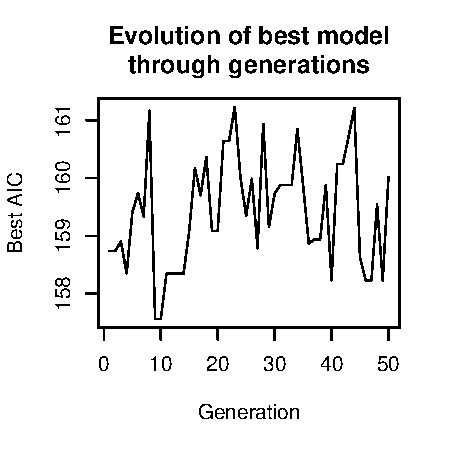
\includegraphics[width=\maxwidth]{figure/latex-unnamed-chunk-4} 


\end{knitrout}

From the plot, we can see that the best model was found at generation 9. 

\section{Contributions} 
\label{sec:contributions}
\subsection{Code writing}
General structure: JRN\\
Functions: JRN, YH

\subsection{Code testing}
Function testing: EB\\
Overall function tests: YH

\subsection{Documentation}
Manual creation: EB\\
Project write-up: Introduction (EB), Code (JRN), Testing (EB, YH)

\section{Appendix}
\label{sec:appendix}
\inputencoding{utf8}
\HeaderA{GA-package}{Genetic algorithm for model variable selection}{GA.Rdash.package}
\keyword{package}{GA-package}
%
\begin{Description}\relax
Final project for Statistics 243. An R package that implements a genetic algorithm for variable selection in linear and GLM problems.
\end{Description}
%
\begin{Details}\relax

\Tabular{ll}{
Package: & GA-package\\{}
Type: & Package\\{}
Version: & 1.0\\{}
Date: & 2014-12-13\\{}
}
\end{Details}
%
\begin{Author}\relax
Eddie Buehler, Yang Hu, JR New
\end{Author}
%
\begin{References}\relax
G. Givens and J. Hoeting. \strong{Computational Statistics, 2nd ed.} (2012).
\end{References}
%
\begin{SeeAlso}\relax
https://github.com/jrnew/genetic-algo
\end{SeeAlso}
%
\begin{Examples}
\begin{ExampleCode}
# Select regression variables for airquality data using lm model and AIC criterion
select_model(
  data = airquality,
  yvar = "Ozone",
  xvars = NULL,
  model = "lm",
  criterion = "AIC",
  pop_size = 100L,
  method_select = "rank",
  method_recombine = "onepoint",
  prob_recombine = 0.6,
  prob_mutate = 0.01,
  num_max_iterations = 100L,
  seed = 123,
  do_parallel = FALSE
)

# With a user-defined model evaluation criterion function
rsquared <- function(lm) {
  mod <- summary(lm)
  return(-mod\$r.squared)
}
ga <- select_model(data = airquality,
                   yvar = "Ozone",
                   model = "lm",
                   criterion = "rsquared",
                   criterion_function = rsquared)
\end{ExampleCode}
\end{Examples}
 
 \inputencoding{utf8}
\HeaderA{select\_model}{Carry out model selection with a genetic algorithm.}{select.Rul.model}
%
\begin{Description}\relax
Main function for carrying out model selection with a genetic algorithm.
\end{Description}
%
\begin{Usage}
\begin{verbatim}
select_model(data, yvar, xvars = NULL, model = "lm", glm_family = NULL,
  criterion = "AIC", pop_size = 100L, method_select = "rank",
  method_recombine = "onepoint", prob_recombine = 0.6, prob_mutate = 0.01,
  num_max_iterations = 100L, seed = 123, do_parallel = FALSE)
\end{verbatim}
\end{Usage}
%
\begin{Arguments}
\begin{ldescription}
\item[\code{data}] Data frame

\item[\code{yvar}] Character; Name of column containing response variable

\item[\code{xvars}] Character vector; Default is all column names that are not yvar;
Name(s) of column(s) containing set of explanatory variables to select on.

\item[\code{model}] Character; "lm" (default) or "glm"; Linear model or
generalized linear model.

\item[\code{glm\_family}] Character if model is "glm", NULL otherwise;
"binomial", "gaussian" (default), "Gamma", "inverse.gaussian", "poisson", "quasi",
"quasibinomial", "quasipoisson"; A family function that gives the error
distribution and link function to be used in the model.

\item[\code{criterion}] "AIC" (default) or "BIC"; Criterion to be minimized.

\item[\code{pop\_size}] Integer; Default is 100; Number of chromosomes per generation.

\item[\code{method\_select}] String; "rank" (linear rank selection) (default) or
"tournament"; Method to select chromosomes for inclusion in mating pool.

\item[\code{method\_recombine}] String; "onepoint" (default), "twopoint", "uniform";
Type of crossover, at one point, at two points or uniformly (at all possible points).

\item[\code{prob\_recombine}] Numeric, between 0 and 1; Default is 0.6;
Probability of recombination.

\item[\code{prob\_mutate}] Numeric, between 0 and 1; Default is 0.01;
Probability of mutation.

\item[\code{num\_max\_iterations}] Non-negative integer; Default is 100;
Maximum number of iterations before algorithm is stopped.

\item[\code{seed}] Non-negative integer; Default is 123; Random seed
for reproducibility.

\item[\code{do\_parallel}] Logical; Default is FALSE; Do in parallel?
\end{ldescription}
\end{Arguments}
 
 \inputencoding{utf8}
\HeaderA{evaluate\_once}{Do evaluation once.}{evaluate.Rul.once}
%
\begin{Description}\relax
Do evaluation for a chromosome by calculating model selection criterion.
\end{Description}
%
\begin{Usage}
\begin{verbatim}
evaluate_once(model_data, xvars_select, model = "lm", glm_family = NULL,
  criterion = "AIC")
\end{verbatim}
\end{Usage}
%
\begin{Arguments}
\begin{ldescription}
\item[\code{glm\_family}] Character if \code{model} is "glm", \code{NULL} otherwise;
"binomial", "gaussian" (default), "Gamma", "inverse.gaussian", "poisson", "quasi",
"quasibinomial", "quasipoisson"; A family function that gives the error
distribution and link function to be used in the model.

\item[\code{model\_data;}] Object of class \code{model\_data}.

\item[\code{xvars\_select;}] Logical vector;

\item[\code{model;}] Character; "lm" (default) or "glm"; Linear model or generalized linear model.

\item[\code{criterion;}] "AIC" (default) or "BIC"; AIC or BIC.
\end{ldescription}
\end{Arguments}
%
\begin{Value}
Numeric; Value of criterion.
\end{Value}
 
 \inputencoding{utf8}
\HeaderA{evaluate}{Do evaluation.}{evaluate}
%
\begin{Description}\relax
Do evaluation for chromosomes in population by calculating model selection criterion.
\end{Description}
%
\begin{Usage}
\begin{verbatim}
evaluate(pop, model_data, model = "lm", glm_family = NULL,
  criterion = "AIC", do_parallel = FALSE)
\end{verbatim}
\end{Usage}
%
\begin{Arguments}
\begin{ldescription}
\item[\code{pop}] Matrix of population of chromosomes.

\item[\code{model\_data}] Object of class model\_data.

\item[\code{model}] Character; "lm" (default) or "glm"; Linear model or
generalized linear model.

\item[\code{glm\_family}] Character if model is "glm", NULL otherwise;
"binomial", "gaussian" (default), "Gamma", "inverse.gaussian", "poisson", "quasi",
"quasibinomial", "quasipoisson"; A family function that gives the error
distribution and link function to be used in the model.

\item[\code{criterion}] "AIC" (default) or "BIC"; Criterion to be minimized.

\item[\code{do\_parallel}] Logical; Default FALSE; Do in parallel?
\end{ldescription}
\end{Arguments}
%
\begin{Value}
Numeric vector; Evaluation values for all chromosomes
in the current generation.
\end{Value}
 
 \inputencoding{utf8}
\HeaderA{initialize}{Initialize first generation of chromosomes.}{initialize}
%
\begin{Description}\relax
Initialize first generation of chromosomes completely randomly.
\end{Description}
%
\begin{Usage}
\begin{verbatim}
initialize(pop_size, num_vars)
\end{verbatim}
\end{Usage}
%
\begin{Arguments}
\begin{ldescription}
\item[\code{pop\_size}] Non-negative integer; Number of chromosomes in population.

\item[\code{num\_vars}] Non-negative integer; Number of variables in model under consideration/
number of genes in each chromosome.
\end{ldescription}
\end{Arguments}
%
\begin{Value}
A matrix of size pop\_size x num\_vars with 1's and 0's.
\end{Value}
 
 \inputencoding{utf8}
\HeaderA{mutate}{Mutate genes in the population.}{mutate}
%
\begin{Description}\relax
Mutate each gene in the population at a pre-defined rate.
\end{Description}
%
\begin{Usage}
\begin{verbatim}
mutate(pop, prob_mutate = 0.01)
\end{verbatim}
\end{Usage}
%
\begin{Arguments}
\begin{ldescription}
\item[\code{pop}] Matrix; Population of chromosomes.

\item[\code{prob\_mutate}] Numeric, between 0 and 1; Default is 0.01; Probability of mutation.
\end{ldescription}
\end{Arguments}
%
\begin{Value}
Matrix of population of chromosomes that have undergone mutation.
\end{Value}
 
 \input{texforfunctions/plot_ga.tex} 
 \inputencoding{utf8}
\HeaderA{process\_data}{Process data for input into genetic algorithm.}{process.Rul.data}
%
\begin{Description}\relax
Process data for input into genetic algorithm.
\end{Description}
%
\begin{Usage}
\begin{verbatim}
process_data(data, yvar, xvars = NULL)
\end{verbatim}
\end{Usage}
%
\begin{Arguments}
\begin{ldescription}
\item[\code{data}] Data frame

\item[\code{yvar}] Character; Name of column containing response variable.

\item[\code{xvars}] Character vector; Default is all column names that are not yvar;
Name(s) of column(s) containing set of explanatory variables to select on.
\end{ldescription}
\end{Arguments}
%
\begin{Value}
A list object named model\_data containing:
\begin{description}

\item[data] Data frame; Processed data with only relevant columns.
\item[yvar] Character; Name of column containing response variable.
\item[xvars] Character vector; Name(s) of column(s) containing
set of explanatory variables to select on.
\item[num\_vars] Integer; Length of xvars.

\end{description}

\end{Value}
 
 \inputencoding{utf8}
\HeaderA{recombine\_once}{Recombine once.}{recombine.Rul.once}
%
\begin{Description}\relax
Carry out crossover of two parent chromosomes to produce one child chromosome.
\end{Description}
%
\begin{Usage}
\begin{verbatim}
recombine_once(parent1, parent2, method = "onepoint")
\end{verbatim}
\end{Usage}
%
\begin{Arguments}
\begin{ldescription}
\item[\code{parent1}] Integer vector of 1st parent chromosome containing 1's and 0's.

\item[\code{parent2}] Integer vector of 2nd parent chromosome containing 1's and 0's.

\item[\code{method}] String; "onepoint" (default), "twopoint", "uniform";
Type of crossover, at one point, at two points or uniformly (at all possible points).
\end{ldescription}
\end{Arguments}
%
\begin{Value}
Integer vector of child chromosome containing 1's and 0's.
\end{Value}
 
 \inputencoding{utf8}
\HeaderA{recombine}{Recombine.}{recombine}
%
\begin{Description}\relax
Carry out crossover of parent chromosomes in a mating pool.
\end{Description}
%
\begin{Usage}
\begin{verbatim}
recombine(pop_mating, pop_size, method = "onepoint", prob_recombine = 0.6,
  do_parallel = FALSE)
\end{verbatim}
\end{Usage}
%
\begin{Arguments}
\begin{ldescription}
\item[\code{pop\_mating}] Matrix of population of chromosomes that form the mating pool.

\item[\code{pop\_size}] Integer; Number of chromosomes in a generation.

\item[\code{method}] String; "onepoint" (default), "twopoint", "uniform";
Type of crossover, at one point, at two points or uniformly (at all possible points).

\item[\code{prob\_recombine}] Numeric, between 0 and 1; Default is 0.6;
Probability of recombination.

\item[\code{do\_parallel}] Logical; Default FALSE; Do in parallel?
\end{ldescription}
\end{Arguments}
%
\begin{Value}
Matrix of population of chromosomes resulting from recombination.
\end{Value}
 
 \inputencoding{utf8}
\HeaderA{reproduce}{Wrapper function for reproduction stage.}{reproduce}
%
\begin{Description}\relax
Wrapper function for reproduction stage.
\end{Description}
%
\begin{Usage}
\begin{verbatim}
reproduce(ga, iteration, do_parallel = FALSE)
\end{verbatim}
\end{Usage}
%
\begin{Arguments}
\begin{ldescription}
\item[\code{ga}] Object of class ga.

\item[\code{iteration}] Iteration number.
\end{ldescription}
\end{Arguments}
%
\begin{Value}
Updated ga list object.
\end{Value}
 
 \inputencoding{utf8}
\HeaderA{select}{Select chromosomes for recombination.}{select}
%
\begin{Description}\relax
Select chromosomes for recombination based on fitness.
\end{Description}
%
\begin{Usage}
\begin{verbatim}
select(pop, evaluation, method = "rank", do_parallel = FALSE)
\end{verbatim}
\end{Usage}
%
\begin{Arguments}
\begin{ldescription}
\item[\code{pop}] Matrix; Population of chromosomes.

\item[\code{evaluation}] Numeric vector; Evaluation values of all chromosomes in population.

\item[\code{method}] String; "rank" (linear rank selection) (default) or
"tournament"; Method to select chromosomes for inclusion in mating pool.

\item[\code{do\_parallel}] Logical; Default \code{FALSE}; Do in parallel?
\end{ldescription}
\end{Arguments}
%
\begin{Value}
Matrix of population of chromosomes that form the mating pool.
\end{Value}
 
 \input{texforfunctions/summary_ga.tex} 


\end{document}
